Die bisher vorgestellten Ansätze arbeiten mehrheitlich über einen \textbf{trusted anonymizer}, der als Middleware zwischen User und LBS agiert und die Anonymisierung übernimmt. Der Vorteil bei der Verwendung von Dummy Trajectories - also falschen Positionsdaten - besteht darin, dass es sich hierbei um einen \textbf{Client-basierten Ansatz} handelt. Der User ist somit für den Schutz seiner Privatsphäre selbst verantwortlich und damit auch nicht abhängig von der Sicherheit und Erreichbarkeit des trusted anonymizers (mit Ausnahme von optionaler Middleware wie in \ref{para:middle} zu sehen) oder der Verfügbarkeit einer ausreichenden Anzahl an Usern in der Umgebung für z.B. k-anonymity Ansätze. Der Grad des Privatsphäreschutzes ist bei dieser Methode vor allem bedingt durch die Anzahl der generierten Dummies, welche in Abhängigkeit zu dem gewünschten Anonymitätsgrad und der zur Verfügung stehenden Processing Power gewählt werden muss.\\
Der Einsatz von Dummy Trajectories hat jedoch auch einige Nachteile. Zum einen entsteht ein Overhead bei jeder Anfrage, da sowohl beim User als auch bei den LBS zusätzliche Ressourcen für Erstellung und Bearbeitung der Dummies benötigt werden. Abhängig von der Art des LBS können auch andere negative Effekte auftreten \cite{Beresford2005}: Durch den Overhead durch Dummies kann zum einen die Kapazität für andere, reale User eingeschränkt werden, zum anderen ist ein Einsatz der Methode bei LBS, welche pro Anfrage abrechnen, zu vermeiden. Auch bei LBS, die beispielsweise Kapazitäten überwachen (z.B. Verfügbarkeit von Parkplätzen oder Auslastung eines Raumes) ist ein Einsatz von Dummies kritisch, da hierdurch die realen Zustände verfälscht werden.\\
Im Gegensatz zu Dummy Positionen ist die Generierung von realistischen Dummy Trajectories, die nicht von realen Trajectories unterschieden werden können, relativ anspruchsvoll \cite{Beresford2003}. Allerdings ist gerade dieser Aspekt sehr wichtig, da durch die Anwendung von Data Mining Techniken auf über längere Zeit gesammelte Trajectories Rückschlüsse auf die realen Trajectories geschlossen werden können. 

\subsubsection{Privatsphäre-Parameter \cite{You2007, Lei2012}} \label{subsubsection:dgparameter}
Es werden drei Parameter vorgeschlagen, mit denen der User den Grad seiner Privatsphäre messen und bestimmten kann:
	\paragraph{Short-term or Snapshot Disclosure (SD)} Basiert auf der aktuellen Position des Users und der Dummies und stellt die Wahrscheinlichkeit dar, dass die reale Position des Users identifiziert werden kann und soll unter einem spezifizierten Schwellenwert liegen. Hierbei ist m die Nummer von Zeitslots in einer Trajectory, \textit{D$_{i}$} ist die das Set von realen und Dummy Trajectories zur Zeit \textit{i} und \textit{|D$_{i}$|} ist die Größe von \textit{D$_{i}$}.
	\begin{equation}
	\label{equation:SD}
	\frac{1}{m} \sum{i=1}{m}{\frac{1}{\left\lvert D_{i} \right\rvert}}
	\end{equation}	
	
	\paragraph{Long-term or Trajectory Disclosure (LD)} Die Wahrscheinlichkeit, die reale Trajectory zwischen allen vorhandenen Trajectories zu identifizieren. Basierend auf der realen Trajectory des Users und den Dummy Trajectories sollte diese unter einem spezifizierten Schwellenwert liegen. \textit{k} sind hierbei die Trajectories, die sich mit anderen überschneiden, und \textit{(n - k)} sind alle Trajectories, die keine Überschneidung haben. \textit{T$_{k}$} ist die Anzahl aller möglichen Trajectories gegeben \textit{k} Trajectories.
	\begin{equation}
	\label{equation:LD}
	\frac{1}{T_{k} + \left( n - k \right)}
	\end{equation}	
	
	\paragraph{Distance Deviation (DD)} Die durchschnittliche Distanz zwischen den Trajectories, wobei \textit{dist(PL$_{i}^{j}$, L$_{dk}^{j}$)} die euklidische Distanz zwischen zwei Punkten \textit{PL, P} angibt. Basierend auf der realen Trajectory des Users und den Dummy Trajectories soll der durchschnittliche Distanzunterschied, also die Distanzabweichung unter den Trajectories, über einem spezifizierten Schwellenwert liegen.
	\begin{equation}
	\label{equation:DD}
	\frac{1}{m} * \frac{1}{n} * \sum{k=1}{n}{\sum{j=1}{m}{dist\left(PL_{i}^{j}, L_{dk}^{j}\right)}}
	\end{equation}	

\subsubsection{Ansätze für die Anonymisierung mit Dummies} \label{subsubsection:realdummy}
Im Folgenden werden einige Anonymisierungstechniken vorgestellt, die auf der Generierung von Dummies basieren, wobei das grundlegende Vorgehen bei allen vorgestellten Ansätzen nahezu gleich ist. Im Folgenden wird der Ablauf bei einer Anfrage mit Dummy Trajectories an ein LBS anhand eines der drei vorgestellten Ansätze geschildert \cite{Kido2005}:\\ 
Der Schutz der Privatsphäre basiert auf einem Set von Dummies, welche der User zusammen mit der realen Position übermittelt. Der User schickt eine Nachricht S an den LBS, welche die Form \textit{S = (u, L$_{1}$, L$_{2}$,..., L$_{m}$)} hat, wobei \textit{u} die ID des Users ist und mit L die reale Position sowie m-1 Dummies angegeben werden. Der LBS übermittelt daraufhin eine Antwort R, bei der für jede der Positionen die dazugehörigen Informationen D$_{x}$ enthalten sind: \textit{R = ((L$_{1}$, D$_{1}$), (L$_{2}$, D$_{2}$),..., (L$_{m}$, D$_{m}$))}. Der User, der sich seiner realen Position bewusst ist, sucht sich nun aus R die erforderlichen Informationen D aus und verwirft die Resultate der übermittelten Dummies. Somit ist gewährleistet, dass der User der Position angepasste Informationen erhält, der LBS jedoch gleichzeitig nicht auf die reale Position des Users schließen kann.

\paragraph{Ansatz: Realitätsnahe Dummy Trajectories \cite{Kido2005}} \label{para:simple}
Dieser Ansatz konzentriert sich auf die Generierung von realitätsnahen Dummies. Wenn die Dummies willkürlich erzeugt werden - also anders als die Positionen und Bewegungen des Nutzers nicht von durch die Umgebung vorgegebene Faktoren (z.B. Bewegungsgeschwindigkeit, Wege und Straßen) eingeschränkt werden - ist die Chance hoch, dass sie auch als Dummies identifiziert werden können. Um dies zu vermeiden werden im Paper zwei verschiedene Algorithmen zur Dummy-Erzeugung vorgestellt - \textbf{Moving in a Neighborhood} und \textbf{Moving in a Limited Neighborhood} - welche in \ref{subsubsection:dgschema} näher vorgestellt werden. Um den Overhead bei dieser Technik zu reduzieren, und damit die Performanz zu verbessern, werden außerdem durch zusätzliche Maßnahmen die Kommunikationskosten gesenkt.

\paragraph{Ansatz: Front-end Modul \cite{Lu2008}} \label{para:modul}
Für den PAD-Ansatz wird zusätzlich zu den Client-seitig generierten Locations ein leichtgewichtiges front-end Modul auf Serverseite vor der eigentlichen Suchmaschine integriert, welche die erhaltenen Positionen effizient verarbeitet. Zusätzlich dazu wird ein kompaktes Format für die übermittelten Locations entwickelt, um den Overhead niedrig zu halten. Die Dummies werden, wie in \ref{subsubsection:dgschema} dargestellt, durch die \textbf{Circle-Based Dummy Generation} und die \textbf{Grid-Based Dummy Generation} erstellt.

\paragraph{Ansatz: Pseudonyme und Middleware \cite{Sahu2012}} \label{para:middle}
Ein anderer Ansatz, um die Privatsphäre von LBS-Usern zu gewährleisten, wird durch die Kombination von Dummy Locations mit einem Application Server realisiert. Hierbei gibt es einige Ähnlichkeiten mit den Mix Zones \cite{Beresford2003}, bei denen User über Middleware anonymisiert werden, indem sie für die Aufenthaltsdauer in einem definierten räumlichen Bereich ein Pseudonym annehmen und auf Positionsupdates verzichten. Somit kann der User nicht von anderen Personen in der Mix Zone differenziert werden, und es ebenso ist keine Verbindung zwischen dem Eintritt und Exit eines Users aus der Mix Zone herstellbar. Es ergibt sich jedoch der Nachteil, dass durch die nicht akkurate Positionsangabe auch die Qualität der LBS abnimmt.\\
Bei dem im Paper vorgeschlagenen Ansatz wird ebenfalls Middleware eingesetzt, welche dem User Pseudonyme zuweist, die jeweils nach einem bestimmten Zeitraum geändert werden. Anders als bei den Mix Zones übermittelt der User jedoch weiterhin Positionsupdates an die LBS, um einen bestmöglichen Service zu erhalten. Jedoch ist dadurch der alleinige Einsatz von mehreren aufeinander folgenden Pseudonymen für die Privatsphäre nicht ausreichend, da durch Inferenz eine Verknüpfung zwischen den Datensätzen hergestellt werden könnte. Deshalb kommen Dummies zum Einsatz, welche zusätzlich zu der realen Position über die Middleware an die LBS übermittelt werden. Mit diesem Vorgehen steht den LBS einerseits eine genaue Position zur Verfügung, um Ergebnisse für die Anfrage zu generieren, gleichzeitig bleibt die Identität des Users jedoch unbekannt.

\subsubsection{Dummy-Generation-Schemata \cite{You2007, Lei2012, Kido2005}} \label{subsubsection:dgschema}
Im folgenden Abschnitt werden einige Algorithmen zur Generierung von Dummies vorgestellt und verglichen.
	\paragraph{Moving in a Neighborhood \cite{Kido2005}} Bei dem diesem Algorithmus werden zukünftige Dummies abhängig von der aktuellen Position des Dummies generiert.
	\paragraph{Moving in a Limited Neighborhood} \cite{Kido2005} Der Algorithmus verwendet die selbe Methode, allerdings wird hierbei die Generierung der Dummies zusätzlich durch Daten von anderen Usern beeinflusst. In einer Region, die bereits eine hohe Personendichte besitzt, wird der Dummy neu generiert.
	\paragraph{Random Pattern Scheme \cite{You2007}} Das Verfahren beginnt mit der Auswahl eines Start- und Endpunktes. Abhängig von der Geschwindigkeit des Dummies und drei verschiedenen Bewegungstypen - horizontal, vertikal und eine Kombination beider - werden randomisiert Zellen auf einem Grid ausgewählt und eine Trajectory erstellt. Die verschiedenen generierten Dummy Trajectories werden über eine längere Zeit für die Anonymisierung verwendet, um auch bei einem längeren Beobachtungszeitsaum den Schutz der Privatsphäre zu gewährleisten.
	\paragraph{Intersection Pattern-based Schemes \cite{Lei2012}} Sie verfolgen das Ziel, die Anzahl an Dummies zu reduzieren und gleichzeitig die in \ref{subsubsection:dgparameter} spezifizierten Parameter einzuhalten. Dabei sollen Überschneidungen zwischen Dummies und realen Trajectories entstehen, wie bei den beiden folgenden Methoden zu sehen ist.\\
	Bei der \textbf{Rotation Dummy Generation} werden Dummies erstellt, indem die reale User Trajectory um einen Punkt rotiert wird. Dabei entsteht genau ein Überschneidungspunkt des Dummies mit der realen Trajectory. Da resultierenden Dummies den festgelegten Parametern SD, LD und DD entsprechen sollen, werden sie zuerst basierend auf DD generiert, indem der Rotationspunkt und -winkel variiert wird. Die resultierenden Dummies werden anschließend nach SD und LD ausgewertet, um ein Set der n besten Dummies zu erhalten, welches für die Anonymisierung verwendet wird. Damit erreichen wir, dass die benötigte Nummer an Dummies reduziert wird, während gleichzeitig die Privatsphäre-Parameter eingehalten werden.\\
	Bei dem \textbf{K-intersected Dummy Generation} Schema existieren mehrere Überschneidungspunkte \textit{k}, wobei \textit{k} vom User bestimmt werden kann. Die einzelnen Dummies werden durch einer Kombination des \textbf{Random Pattern Scheme} und der \textbf{Rotation Dummy Generation} erstellt. Die Pfade zwischen zwei Überschneidungen werden durch das \textbf{Random Pattern Scheme} generiert, die Pfade nach den Überschneidungspunkten entstehen durch \textbf{Rotation Dummy Generation}, wie in \ref{fig_Lei2012KD} zu sehen.
	\begin{figure}[!h]
		\centering
		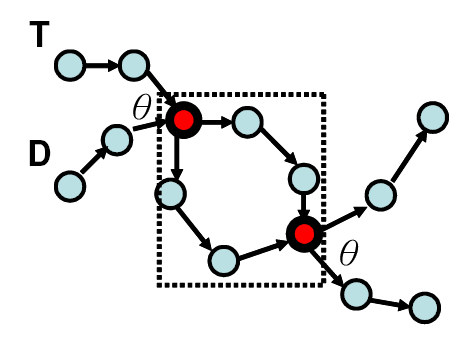
\includegraphics[width=3cm]{Bilder/Lei2012KD.png}
		\caption{K-intersected Dummy Generation, Source: \protect\cite{Lei2012}}
		\label{fig_Lei2012KD}
	\end{figure}
	\paragraph{Circle-Based Dummy Generation \cite{Lu2008}} Diese Methode fokussiert sich auf die Wahrung der Privatsphäre von Snapshots, also einzelner Positionen von Nutzern, und nicht von Trajectories. Eine Anwendung auf Trajectories, die ja eine Sequenz von Positionen darstellen, ist natürlich ebenfalls möglich. Die vom Algorithmus erzeugten Dummies sowie die reale Position liegen dabei alle innerhalb eines Kreises, wobei der Radius sowie der Mittelpunkt durch entsprechende Parameter randomisiert bestimmt wird. Die Winkel zwischen den verschieden Positionen k sind äquivalent und von der Anzahl der Positionen abhängig.
	\paragraph{Grid-Based Dummy Generation \cite{Lu2008}} Hierbei wird ein uniformes, quadratisches Grid mit k Eckpunkten erzeugt, von denen einer der realen Position des Users entspricht. Die k-1 erzeugten Eckpunkte dienen als Dummies für die Anfrage an LBS.
	\begin{figure}[!h]
		\centering
		\subfloat[A]{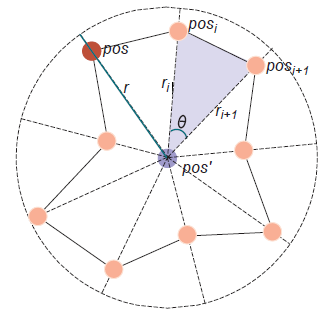
\includegraphics[width=4.4cm]{Bilder/Lu2008CD.png}\label{figA}}
		\subfloat[B]{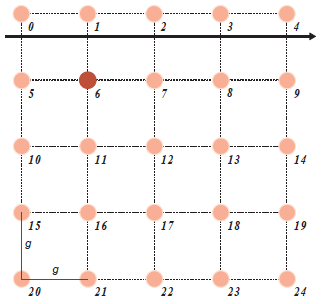
\includegraphics[width=4.4cm]{Bilder/Lu2008GD.png}\label{figB}}
		\caption{Circle- und Grid-based Dummy Generation, Source: \protect\cite{Lu2008}}
		\label{fig_Lu2008}
	\end{figure}
	\paragraph{Pause-Based Dummy Generation \cite{Kato2012}}
	Bei den bisherigen Verfahren werden Umweltbedingungen (z.B. unbegehbares Gelände) und menschliches Verhalten (z.B. Pausen bei Sehenswürdigkeiten), welche Trajectories beeinflussen, gar nicht oder nur in geringem Ausmaß bei der Generierung von Dummy Trajectories beachtet, weshalb diese unter Umständen leicht identifizierbar sind. Bei dieser Methode werden möglichst natürliche Dummies erzeugt, indem basierend auf bekannten Trajectories Pausenpositionen integriert werden.

Im Vergleich zur Circle- oder Grid-based Dummy Generation sind Dummies, die durch Random Pattern Schemes oder Intersection Pattern-based Schemes entstanden sind, aufgrund ihres kontinuierlichen Verlaufs besser geeignet, um die Privatsphäre des Users gegen Data Mining und längerfristige Beobachtung zu schützen. Am effizientesten sind jedoch die Moving in a (Limited) Neighborhood und der Pause-Based Dummy Generation Algorithmus, da sie realen Trajectories von Usern sehr ähnlich sind \cite{Kukkapalli2012}. 